\documentclass[tikz,border=10pt]{standalone}
% Shared preamble for the CenterTask panel files (panel_a/b/c.tex).
% Edit colours and node styles here, once.
\usepackage{amsmath}
\usetikzlibrary{arrows.meta,positioning,calc}

% category colours as in ColorCategoryMap.m: 1=Short/Orange, 2=Mid/Green, 3=Long/Blue
\definecolor{catShort}{RGB}{243,178,132}
\definecolor{catMid}{RGB}{158,209,172}
\definecolor{catLong}{RGB}{157,188,234}

\tikzset{ctpanel/.style={
  font=\sffamily,
  band/.style={rounded corners=6pt, fill=black!7, draw=none, inner sep=8pt, minimum height=1.15cm},
  unit/.style={circle, fill=catMid!60, draw=none, minimum size=0.95cm, inner sep=0pt},
  flow/.style={-{Latex[length=2.2mm]}, line width=0.8pt},
  rowlab/.style={anchor=east, font=\sffamily\large},
  now/.style={fill=catShort!55, rounded corners=3pt, inner sep=3pt},
  stage/.style={rounded corners=6pt, fill=black!8, draw=none, inner sep=8pt, minimum height=1.2cm, align=center},
  target/.style={circle, minimum size=0.9cm, inner sep=0pt, draw=none, font=\sffamily\scriptsize, text=black!75},
  axis/.style={line width=0.6pt},
}}


% ---------------------------------------------------------------------
%  One GRU cell (Cho et al. 2014), as used by the trial-level tiny RNN
%  and by the motor network. Reset gate r_t, update gate z_t, candidate
%  state h~_t, and the interpolation that writes the new state h_t.
% ---------------------------------------------------------------------

\begin{document}
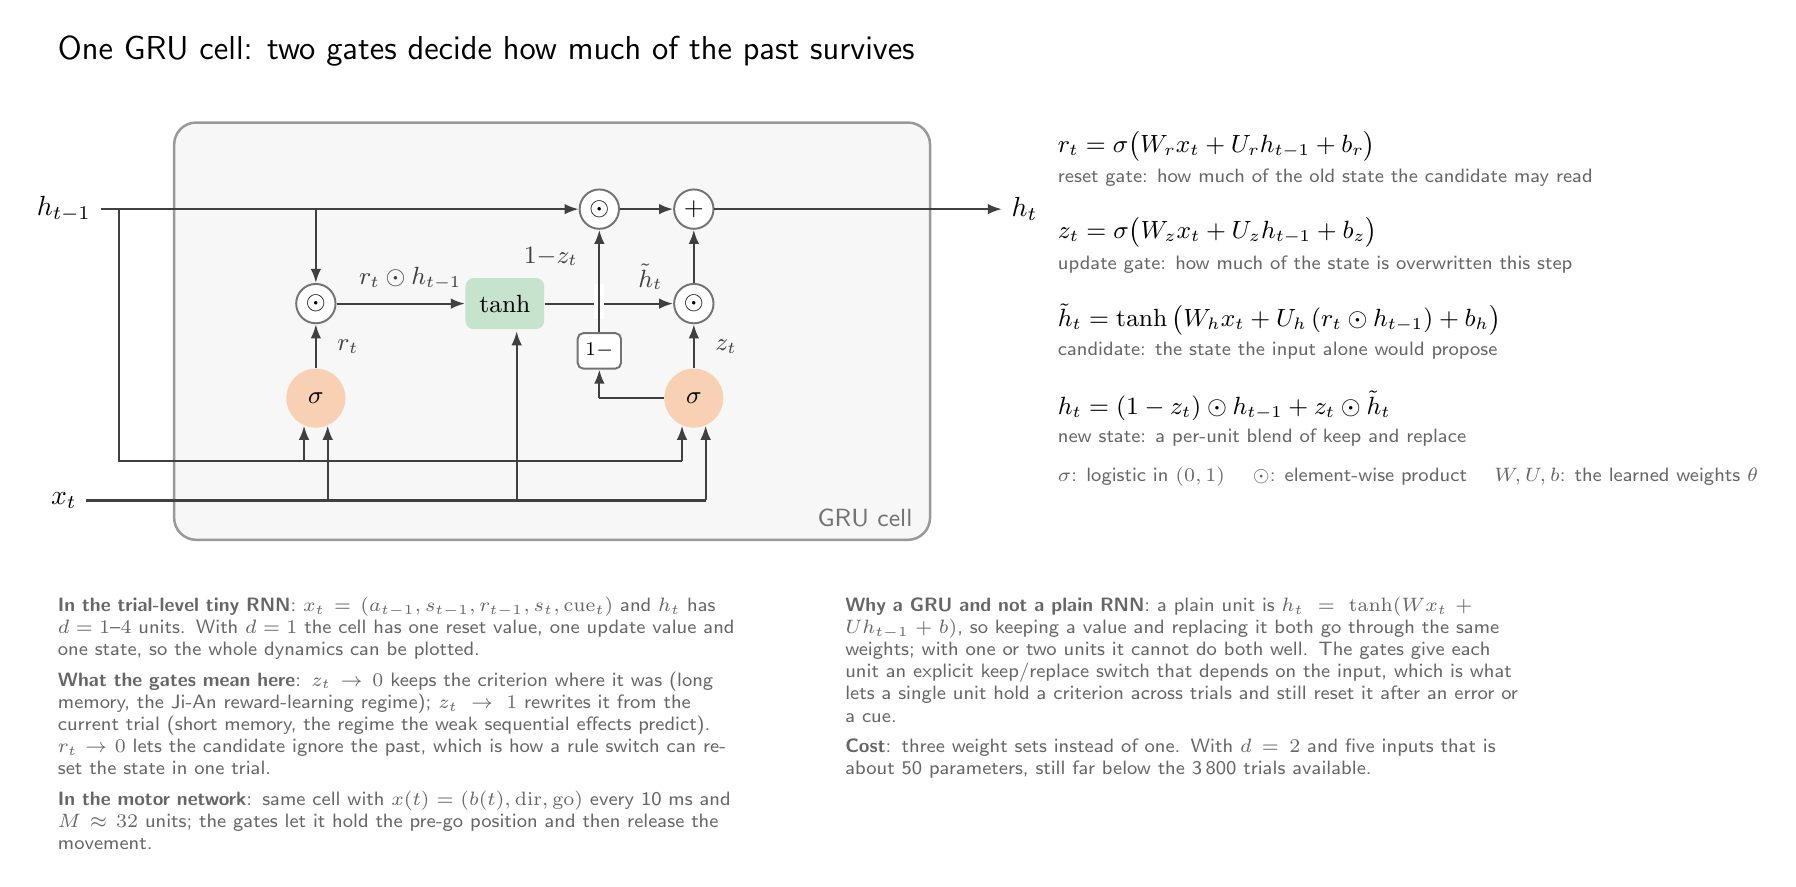
\begin{tikzpicture}[ctpanel,
  cell/.style={rounded corners=8pt, draw=black!40, line width=0.9pt, fill=black!3},
  gate/.style={circle, draw=none, fill=catShort!60, minimum size=0.75cm, inner sep=0pt, font=\small},
  cand/.style={rounded corners=3pt, draw=none, fill=catMid!60, minimum width=1.0cm, minimum height=0.65cm, font=\small},
  op/.style={circle, draw=black!55, line width=0.7pt, fill=white, minimum size=0.5cm, inner sep=0pt, font=\small},
  oneminus/.style={rounded corners=2pt, draw=black!55, line width=0.7pt, fill=white, minimum width=0.55cm, minimum height=0.45cm, inner sep=1pt, font=\scriptsize},
  wire/.style={-{Latex[length=1.8mm]}, line width=0.8pt, black!75},
  bus/.style={line width=0.8pt, black!75},
  siglab/.style={font=\small, text=black!75},
  eq/.style={font=\small, anchor=west},
  note/.style={font=\sffamily\scriptsize, text=black!60, align=left, anchor=north west, text width=8.6cm},
]

\node[font=\sffamily\large, anchor=west] at (-1.8,5.6) {One GRU cell: two gates decide how much of the past survives};

% ---- cell body ----
\draw[cell] (-0.2,-0.6) rectangle (9.4,4.7);
\node[font=\sffamily\small, text=black!55, anchor=south east] at (9.3,-0.55) {GRU cell};

% ---- external ports ----
\node (hprev) at (-1.6,3.6) {$h_{t-1}$};
\node (hnext) at (10.6,3.6) {$h_t$};
\node (xin)   at (-1.6,-0.1) {$x_t$};

% ---- operators on the top line ----
\node[op] (mr)  at (1.6,2.4) {$\odot$};   % r * h_{t-1}
\node[op] (m1)  at (5.2,3.6) {$\odot$};   % (1-z) * h_{t-1}
\node[op] (add) at (6.4,3.6) {$+$};
\node[op] (m2)  at (6.4,2.4) {$\odot$};   % z * h~

% ---- gates and candidate ----
\node[gate] (sr) at (1.6,1.2) {$\sigma$};
\node[cand] (th) at (4.0,2.4) {$\tanh$};
\node[gate] (sz) at (6.4,1.2) {$\sigma$};
\node[oneminus] (om) at (5.2,1.8) {$1{-}$};

% ---- top line: h_{t-1} -> (1-z)*h -> + -> h_t ----
\draw[bus]  (hprev) -- (1.6,3.6);
\draw[wire] (1.6,3.6) -- (m1);
\draw[wire] (m1) -- (add);
\draw[wire] (add) -- (hnext);
\draw[wire] (1.6,3.6) -- (mr);              % h_{t-1} into reset product

% ---- h_{t-1} bus to the gates (left, down, along the bottom) ----
\draw[bus] (-0.9,3.6) -- (-0.9,0.4) -- (6.25,0.4);
\draw[wire] (1.45,0.4) -- (1.45,0.85);
\draw[wire] (6.25,0.4) -- (6.25,0.85);

% ---- x_t bus ----
\draw[bus] (xin) -- (6.55,-0.1);
\draw[wire] (1.75,-0.1) -- (1.75,0.85);
\draw[wire] (4.15,-0.1) -- (4.15,2.05);
\draw[wire] (6.55,-0.1) -- (6.55,0.85);

% ---- reset path ----
\draw[wire] (sr) -- (mr);
\node[siglab, anchor=west] at (1.75,1.85) {$r_t$};
\draw[wire] (mr) -- (th);
\node[siglab, anchor=south] at (2.8,2.45) {$r_t\odot h_{t-1}$};

% ---- candidate -> z * h~ -> + ----
\draw[wire] (th) -- (m2);
\node[siglab, anchor=south] at (5.85,2.45) {$\tilde h_t$};
\draw[wire] (m2) -- (add);

% ---- update path ----
\draw[wire] (sz) -- (m2);
\node[siglab, anchor=west] at (6.55,1.85) {$z_t$};
\draw[bus] (sz) -- (5.2,1.2);
\draw[wire] (5.2,1.2) -- (om);
% bridge over the h~ line
\draw[white, line width=3.5pt] (5.2,2.2) -- (5.2,2.65);
\draw[wire] (om) -- (m1);
\node[siglab, anchor=east] at (5.05,3.0) {$1{-}z_t$};

% ---- equations ----
\node[eq] at (10.9,4.4) {$r_t = \sigma\big(W_r x_t + U_r h_{t-1} + b_r\big)$};
\node[eq, font=\sffamily\scriptsize, text=black!60] at (10.9,4.0) {reset gate: how much of the old state the candidate may read};
\node[eq] at (10.9,3.3) {$z_t = \sigma\big(W_z x_t + U_z h_{t-1} + b_z\big)$};
\node[eq, font=\sffamily\scriptsize, text=black!60] at (10.9,2.9) {update gate: how much of the state is overwritten this step};
\node[eq] at (10.9,2.2) {$\tilde h_t = \tanh\big(W_h x_t + U_h\,(r_t\odot h_{t-1}) + b_h\big)$};
\node[eq, font=\sffamily\scriptsize, text=black!60] at (10.9,1.8) {candidate: the state the input alone would propose};
\node[eq] at (10.9,1.1) {$h_t = (1-z_t)\odot h_{t-1} + z_t\odot \tilde h_t$};
\node[eq, font=\sffamily\scriptsize, text=black!60] at (10.9,0.7) {new state: a per-unit blend of keep and replace};
\node[eq, font=\sffamily\scriptsize, text=black!60] at (10.9,0.2) {$\sigma$: logistic in $(0,1)$ \quad $\odot$: element-wise product \quad $W, U, b$: the learned weights $\theta$};

% ---- notes for our case ----
\node[note] at (-1.8,-1.2) {%
  \textbf{In the trial-level tiny RNN}: $x_t = (a_{t-1}, s_{t-1}, r_{t-1}, s_t, \mathrm{cue}_t)$ and $h_t$ has $d = 1$--$4$ units.
  With $d = 1$ the cell has one reset value, one update value and one state, so the whole dynamics can be plotted.\\[3pt]
  \textbf{What the gates mean here}: $z_t \to 0$ keeps the criterion where it was (long memory, the Ji-An reward-learning regime);
  $z_t \to 1$ rewrites it from the current trial (short memory, the regime the weak sequential effects predict).
  $r_t \to 0$ lets the candidate ignore the past, which is how a rule switch can reset the state in one trial.\\[3pt]
  \textbf{In the motor network}: same cell with $x(t) = (b(t), \mathrm{dir}, \mathrm{go})$ every 10 ms and $M \approx 32$ units;
  the gates let it hold the pre-go position and then release the movement.
};
\node[note, text width=8.6cm] at (8.2,-1.2) {%
  \textbf{Why a GRU and not a plain RNN}: a plain unit is $h_t = \tanh(Wx_t + Uh_{t-1} + b)$, so keeping a value and
  replacing it both go through the same weights; with one or two units it cannot do both well.
  The gates give each unit an explicit keep/replace switch that depends on the input,
  which is what lets a single unit hold a criterion across trials and still reset it after an error or a cue.\\[3pt]
  \textbf{Cost}: three weight sets instead of one. With $d = 2$ and five inputs that is about 50 parameters,
  still far below the 3\,800 trials available.
};

\end{tikzpicture}
\end{document}
